%%%%%%%%%%%%%%%%%%%%%%%%%%%%%%%%%%%%%%%%%
% Jacobs Portrait Poster
% LaTeX Template
% Version 1.0 (31/08/2015)
% (Based on Version 1.0 (29/03/13) of the landscape template
%
% Created by:
% Computational Physics and Biophysics Group, Jacobs University
% https://teamwork.jacobs-university.de:8443/confluence/display/CoPandBiG/LaTeX+Poster
% 
% Further modified by:
% Nathaniel Johnston (nathaniel@njohnston.ca)
% and
% Cameron Smith (@cwsmith on GitHub)
%
% Portrait version by:
% John Hammersley
%
% The landscape version of this template was downloaded from:
% http://www.LaTeXTemplates.com
%
% License:
% CC BY-NC-SA 3.0 (http://creativecommons.org/licenses/by-nc-sa/3.0/)
%
%%%%%%%%%%%%%%%%%%%%%%%%%%%%%%%%%%%%%%%%%

%----------------------------------------------------------------------------------------
%	PACKAGES AND OTHER DOCUMENT CONFIGURATIONS
%----------------------------------------------------------------------------------------

\documentclass[final]{beamer}

\usepackage[size=a1,scale=0.78]{beamerposter} % Use the beamerposter package for laying out the poster

\usetheme{nsfposter} % Use the confposter theme supplied with this template

\setbeamercolor{block title}{fg=ngreen,bg=white} % Colors of the block titles
\setbeamercolor{block body}{fg=black,bg=white} % Colors of the body of blocks
\setbeamercolor{block alerted title}{fg=white,bg=dblue!70} % Colors of the highlighted block titles
\setbeamercolor{block alerted body}{fg=black,bg=dblue!10} % Colors of the body of highlighted blocks
% Many more colors are available for use in beamerthemeconfposter.sty

%-----------------------------------------------------------
% Define the column widths and overall poster size
% To set effective sepwid, onecolwid and twocolwid values, first choose how many columns you want and how much separation you want between columns
% In this template, the separation width chosen is 0.024 of the paper width and a 4-column layout
% onecolwid should therefore be (1-(# of columns+1)*sepwid)/# of columns e.g. (1-(4+1)*0.024)/4 = 0.22

\newlength{\sepwid}
\newlength{\onecolwid}
\setlength{\paperwidth}{24in} % A1
\setlength{\paperheight}{18in} % A1
\setlength{\sepwid}{0.024\paperwidth} % Separation width (white space) between columns
\setlength{\onecolwid}{0.30\paperwidth} % Width of one column
\setlength{\topmargin}{-0.5in} % Reduce the top margin size
%-----------------------------------------------------------

\usepackage{graphicx}  % Required for including images

%algorithms and pseudo code
\usepackage{algorithm}
\usepackage[noend]{algpseudocode}

%----------------------------------------------------------------------------------------
%	TITLE SECTION 
%----------------------------------------------------------------------------------------

\title{Fast Dynamic Load Balancing Tools for Extreme Scale Systems} % Poster title

\author{PI: Mark S. Shephard (shephard@rpi.edu), Co-PI: Cameron W. Smith, Ph.D. Student: Gerrett Diamond} % Author(s)

\institute{Scientific Computation Research Center (SCOREC) at Rensselaer Polytechnic Institute, Troy, NY, USA} % Institution(s)

%----------------------------------------------------------------------------------------

\begin{document}

\addtobeamertemplate{block end}{}{\vspace*{2ex}} % White space under blocks
\addtobeamertemplate{block alerted end}{}{\vspace*{2ex}} % White space under highlighted (alert) blocks

\setlength{\belowcaptionskip}{2ex} % White space under figures
\setlength\belowdisplayshortskip{2ex} % White space under equations

\begin{frame}[t] % The whole poster is enclosed in one beamer frame

\begin{columns}[t] % three columns

\begin{column}{\sepwid}\end{column} % Empty spacer column

\begin{column}{\onecolwid} % The first column

%----------------------------------------------------------------------------------------
%	OBJECTIVES
%----------------------------------------------------------------------------------------

\begin{alertblock}{Motivation and Focus}
  GPUs provide >90\% of the compute power on leadership systems.\\
  Simulations with regions of physical interest that change can have\\
  \begin{itemize}
    \item complex relational structures,
    \item irregular forms of computational \& communication costs, and
    \item evolving imbalance of work characterized by multiple criteria.
  \end{itemize}
  Provide fast dynamic load balancing on GPUs where simulation data exists. \\
  \vskip1cm
  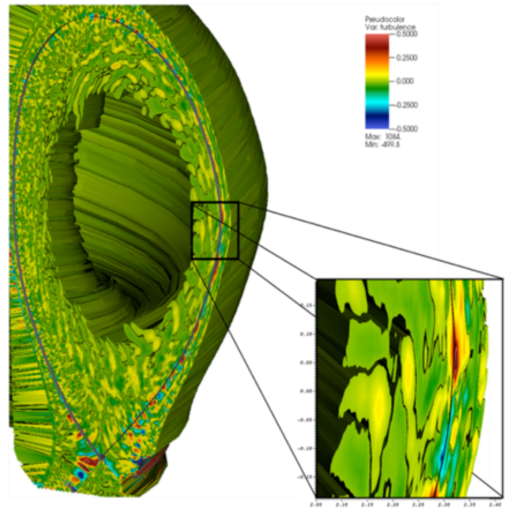
\includegraphics[width=.45\textwidth]{../salishan2019/figures/xgcCase.png}
  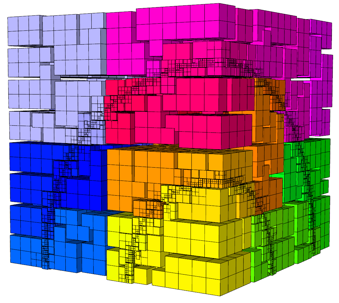
\includegraphics[width=.45\textwidth]{../salishan2019/figures/laghos_sedov.png}\\
  \small{XGC fusion plasma physics (left) and MFEM Laghos Sedov blast
  (right).}
\end{alertblock}

\end{column} % End of the first column
\begin{column}{\sepwid}\end{column} % Empty spacer column
\begin{column}{\onecolwid} % The second column

\begin{block}{Element Partition: Mesh Vertex Imbalance Reduction}
  The partitions before using EnGPar:\\
  \begin{table}[!h]
    \small
    \centering
    \begin{tabular}{||c|c|c|c||}
      \hline
      Number of Parts &128Ki&256Ki&512Ki \\
      \hline
      Elements per part & 9,836 & 4,918&2,459  \\
      \hline
      Vertex imbalance & 1.13 & 1.18 & 1.53 \\
      \hline
      Element imbalance & 1.02& 1.02& 1.02\\
      \hline
    \end{tabular}
  \end{table}
  {\centering
    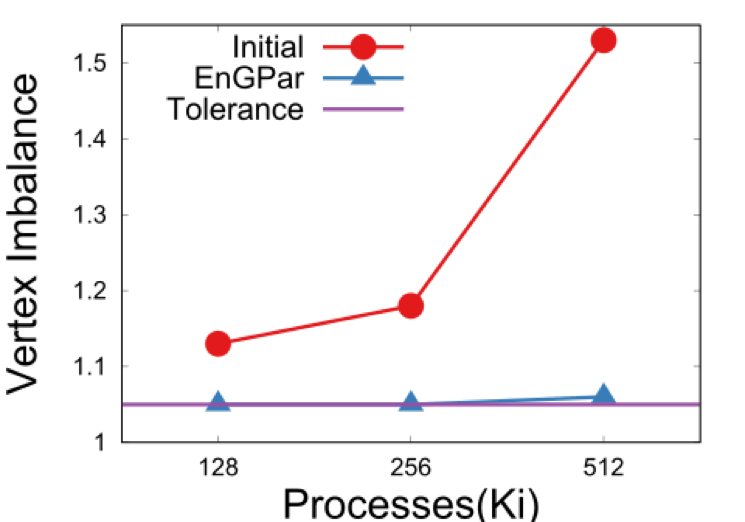
\includegraphics[width=.6\textwidth]{../accelerated_cse19/figures/elmPtn_vtxImb.png}
    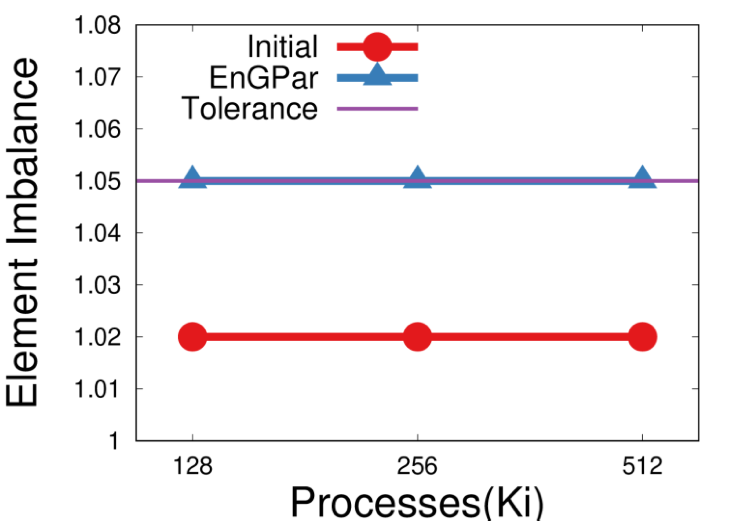
\includegraphics[width=.6\textwidth]{../accelerated_cse19/figures/elmPtn_elmImb.png} \\
    Mesh vertex imbalances are reduced from 13\% to 5\% for 128Ki, 18\% to 5\% for
    256Ki, and 53\% to 6\% for 512Ki.  Edge cut is increased by 1\%.
  }
\end{block}

\end{column} % End of the second column
\begin{column}{\sepwid}\end{column} % Empty spacer column
\begin{column}{\onecolwid} % The third column

\begin{block}{Accelerating BFS with OpenCL and Selection with Kokkos}
  {
    \centering
    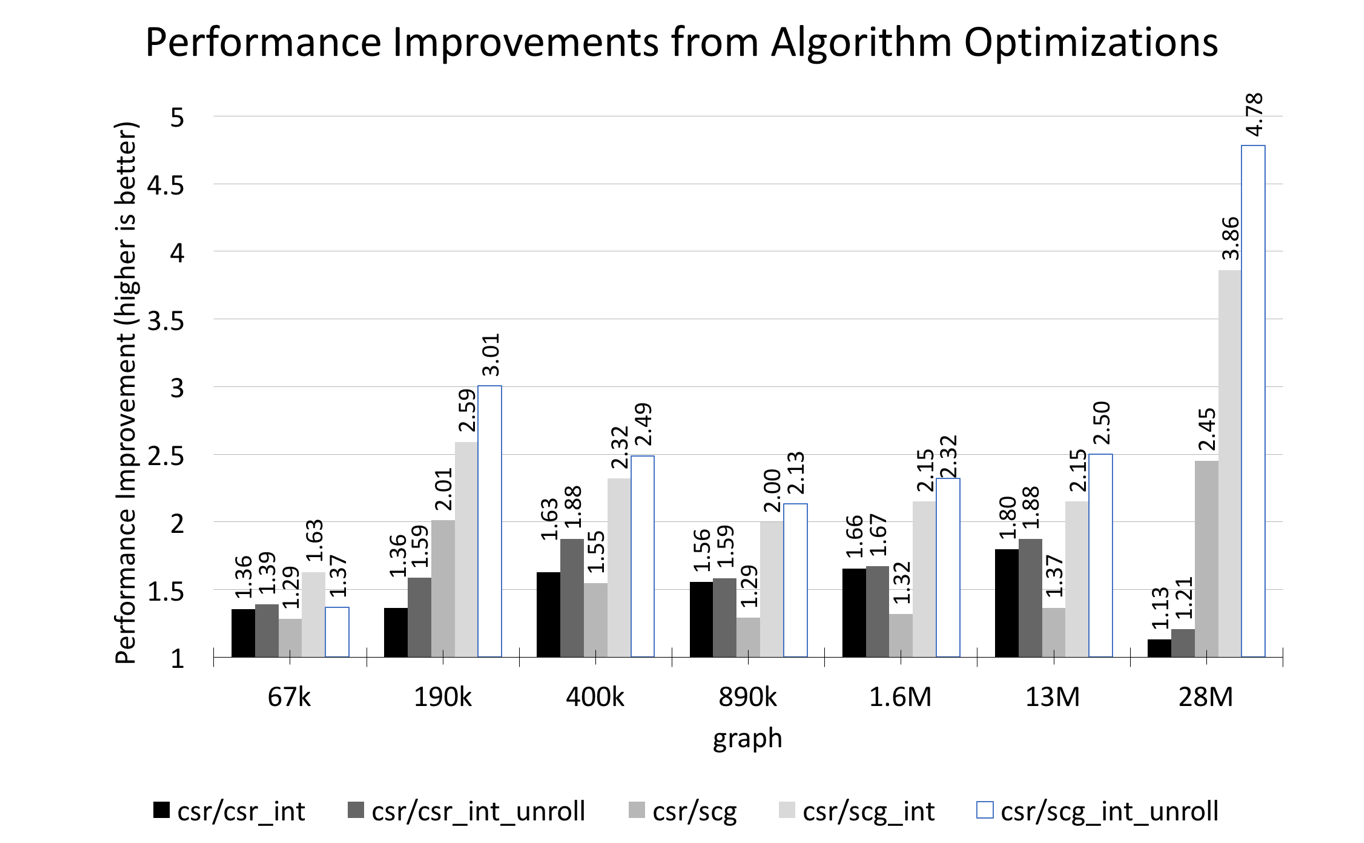
\includegraphics[width=.97\textwidth]{../accelerated_cse19/results/openclBfs.png} \\
    { \small
    \texttt{push}: C++ serial push,
    \texttt{pull}: C++ serial `pull',
    \texttt{csr}: OpenCL `pull' on CSR, 
    \texttt{scg}: OpenCL `pull' on Sell-C-Sigma,
    \texttt{*\_int}: 4B int,
    \texttt{*\_unroll}: unroll the vtx-to-hyperedge loop
    }
  }\\
  { \centering
    Making good decisions \\
    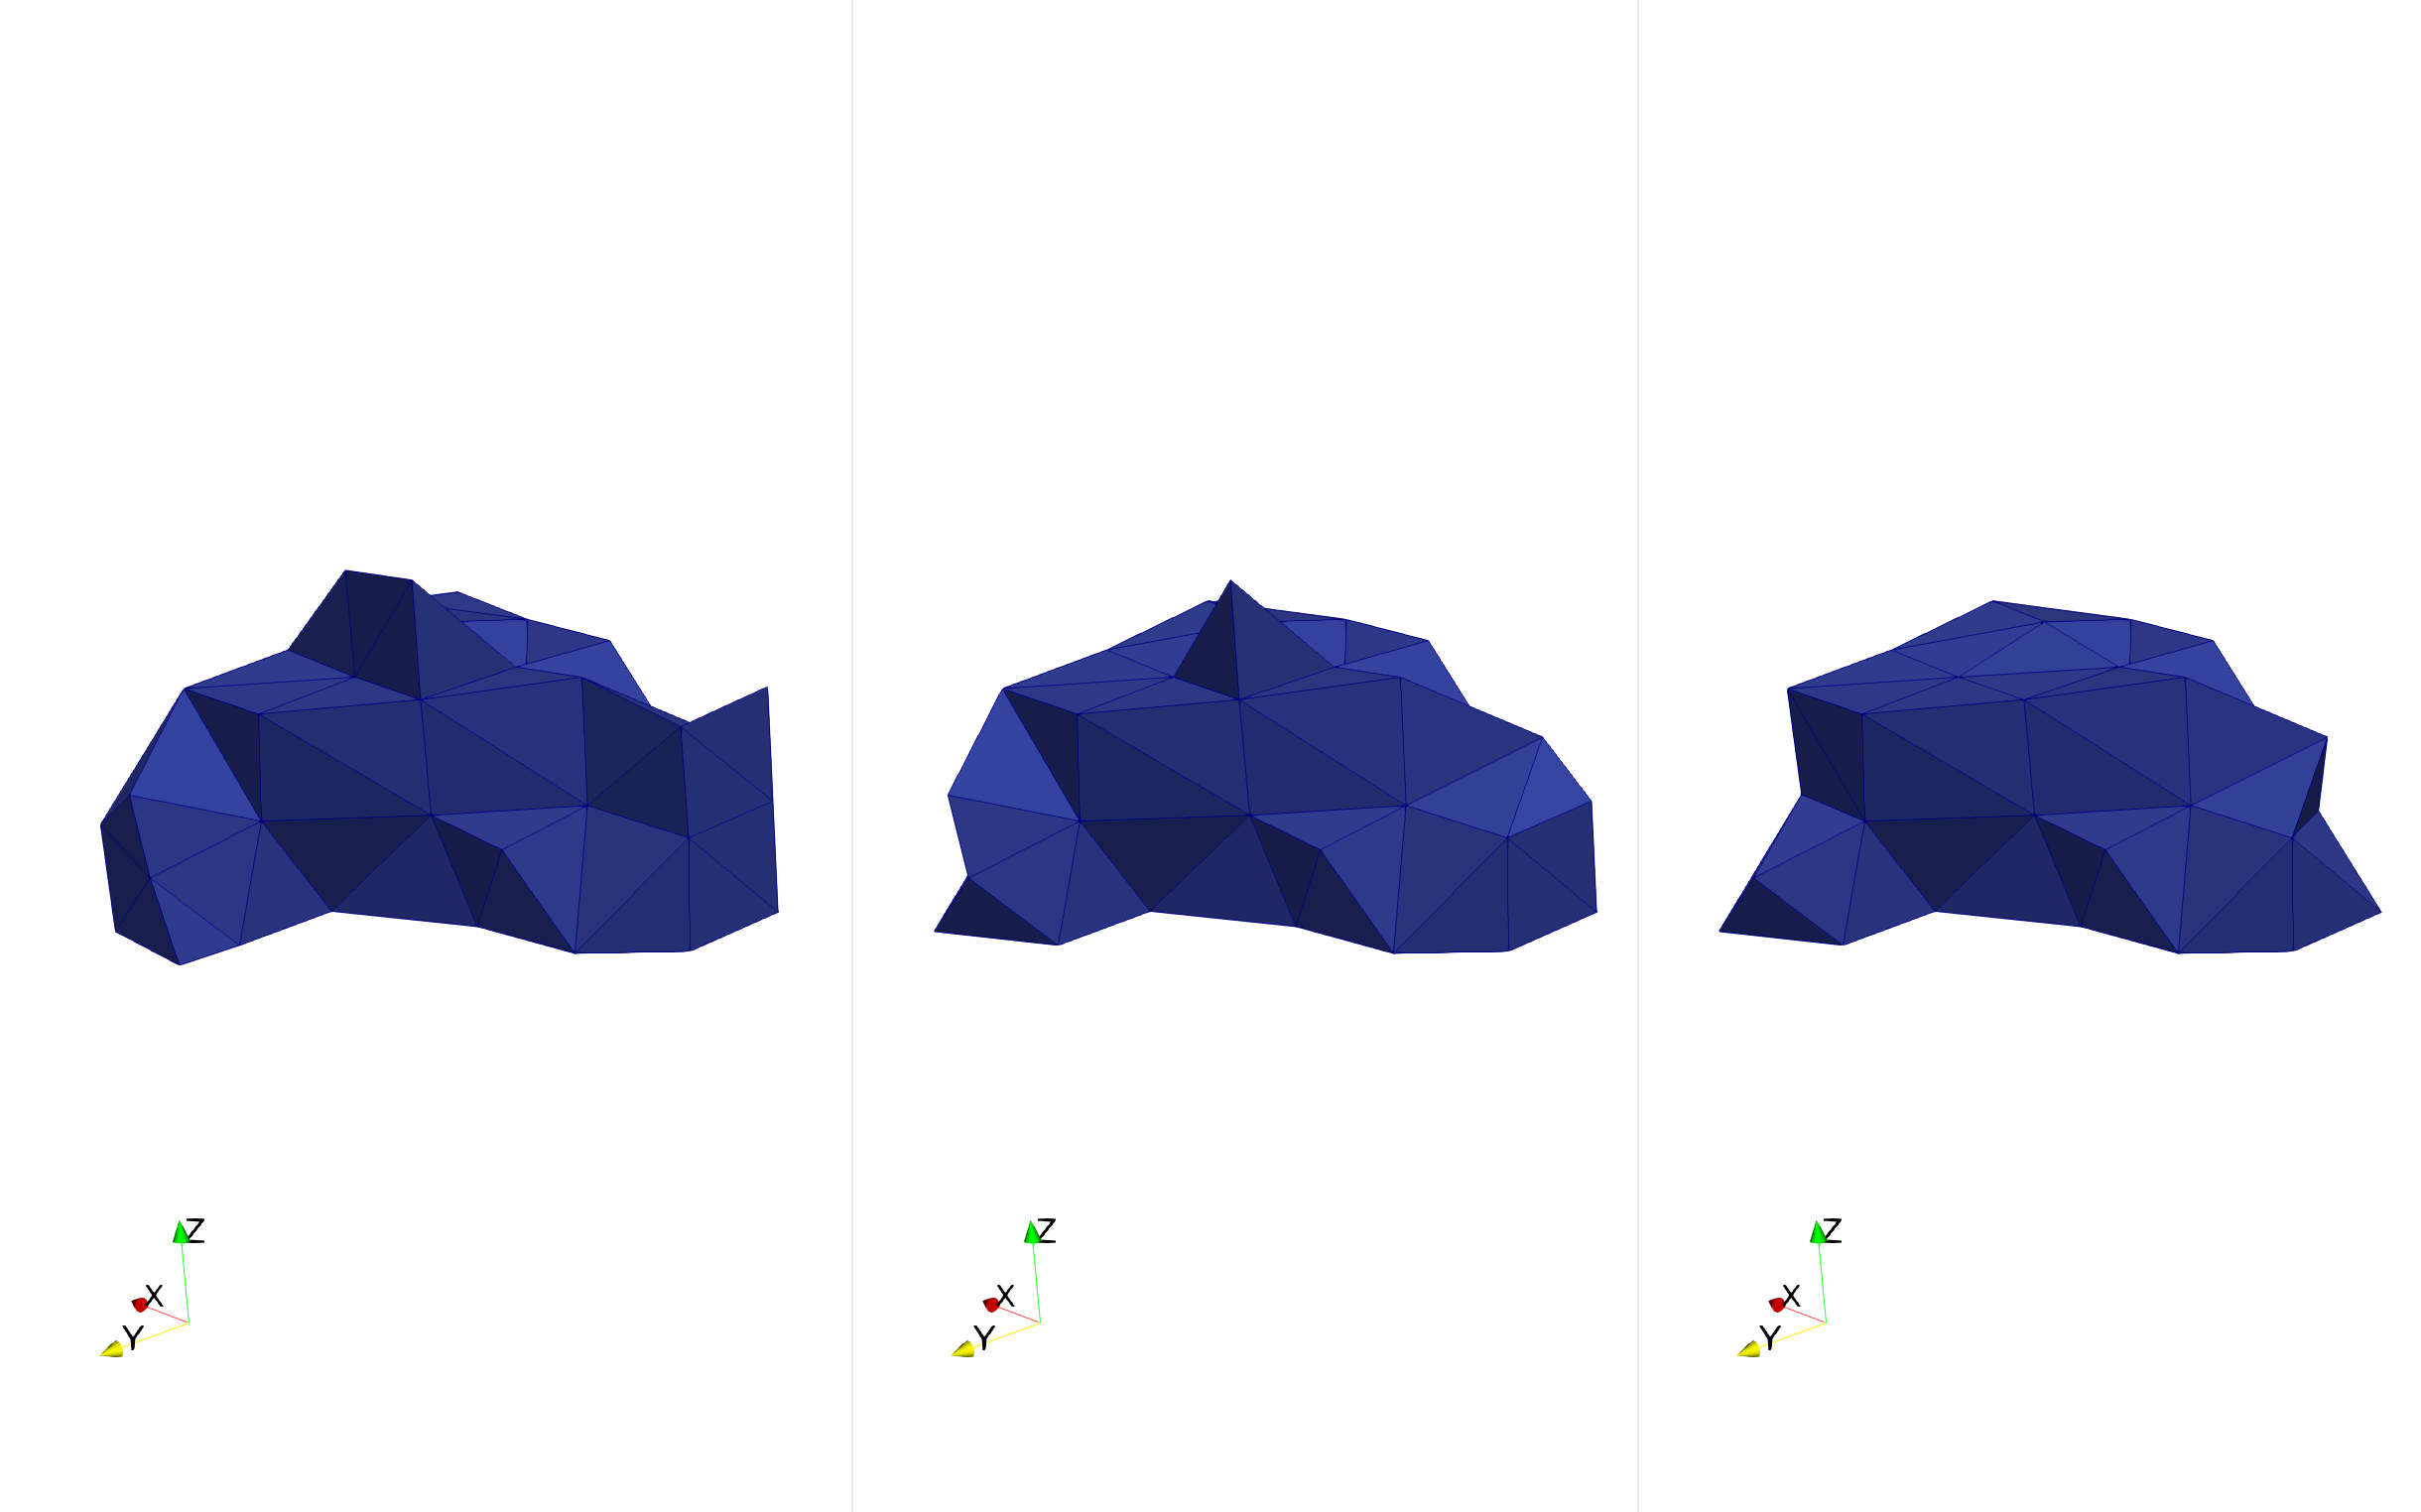
\includegraphics[width=\textwidth]{../accelerated_cse19/figures/selectionEx.png}\\
    Initial, GPU Selection, CPU Selection
  }
  Bias selection towards cavities with highest topological distance.
\end{block}


\end{column} % End of the third column

\begin{column}{\sepwid}\end{column} % Empty spacer column

\end{columns} % End of all the columns in the poster

\end{frame} % End of the enclosing frame

\end{document}
